\documentclass{rapportENSCP}
\usepackage{lipsum}
\usepackage{tabularx} 
\usepackage{xspace}
\usepackage{multirow}
\usepackage{makecell}
\usepackage{graphicx}

\title{Laboratory Internship Report – Template} %Thanks for Rapport CentraleSupelec - Template, By Axel Poupart-Lafarge
\begin{document}
\newcommand{\YGG}{$Y_3Ga_5O_{12}\xspace $ }
\newcommand{\YIG}{$Y_3Fe_5O_{12}\xspace $ }
\newcommand{\YAG}{$Y_3Al_5O_{12}\xspace $ }



%----------- Informations du rapport ---------

\logoentreprise{logos/logoIRCP.png}

\titre{Laboratory internship report} % Titre du fichier

\mention{Experimental laboratory internship} % Nom de la Mention
%\trigrammemention{Master IA} % Pour le bas de la page
\master{Engineering programme} % Nom du master
%\filiere{Filière Management de projet et Transformation} % Nom de la filière

\eleve{Alban Laborde-Laulhé  }

\dates{24 September 2024 – 19 December 2024 }

% Informations tuteurs écoles
\tuteurecole{
    \textsc{Pierre Haquette} \\
    pierre.haquette@chimieparistech.psl.eu
} 

\tuteurentreprise{
    \textsc{Pascal Loiseau} \\
    pascal.loiseau@chimieparistech.psl.eu \\
    \textsc{Alban Ferrier} \\
    alban.ferrier@chimieparistech.psl.eu
}

%----------- Initialisation -------------------
        
\fairemarges %Afficher les marges
\fairepagedegarde %Créer la page de garde

%----------- Abstract -------------------
%\vspace*{\stretch{1}}
%\begin{center}
%	\begin{abstract}
%        \lipsum[1]
%        \rule{\linewidth}{0.2 mm} \\[0.4 cm]
%        \begin{center}\textbf{Summary :}\end{center} 
%        \lipsum[2]
%    \end{abstract}
%\end{center}
%\vspace*{\stretch{1}}
%\newpage

%------------ Table des matières ----------------
\setcounter{figure}{0}


\textit{This report has been translated from French into English using automated tools; despite careful review, translation errors may remain.}

\tabledematieres % Créer la table de matières

%------------ Corps du rapport ----------------

%------------ Introduction ----------------

\section{Acknowledgements} 
First of all, I would like to warmly thank my two supervisors, Pascal Loiseau and Alban Ferrier, for their guidance throughout this internship. Their patience, teaching skills and availability, despite very busy schedules, were invaluable in answering my many questions and assisting me during my first experimental manipulations.

I would also like to express my gratitude to the whole MPOE team for their warm welcome, and in particular to Slimane Raissi for his kindness, his always clear explanations and his precious help in monitoring certain experiments when I was not available, as well as to Nicolas Caraud for his patience and insightful advice on the operation of the various instruments in the laboratory. Many thanks as well to Alix Guerber for her energy and good humour, and to Jean-François Engrand who, besides having an answer to almost any problem, also knows how to hit things very hard—which is practical when you need to break stuff.

I am also grateful to all the IRCP staff, who welcomed me warmly and provided precious support throughout these three months. Finally, I would like to thank Pierre Haquette and Philippe Vernazobres, representatives of the school, who enabled me to carry out this internship within this wonderful team.

\newpage

\section{Abbreviations}
\begin{itemize}
    \item \textbf{YAG: } Yttrium Aluminium Garnet (\YAG)
    \item \textbf{YGG: } Yttrium Gallium Garnet (\YGG)
    \item \textbf{YIG: } Yttrium Iron Garnet (\YIG)
    \item \textbf{YIGG: } Mixture containing 50 mol\% YGG and 50 mol\% YIG
    \item \textbf{XRD: } X-ray diffraction (diffraction des rayons X)
\end{itemize}

\section{Abstract}
This report presents the results of an experimental internship carried out in the MPOE laboratory of the IRCP at Chimie ParisTech, focusing on flux growth of yttrium garnets, in particular YIG ($Y_3Fe_5O_{12}$) and YGG ($Y_3Ga_5O_{12}$). The main objective was to assess the feasibility and optimal conditions for the growth of these garnets in two different flux systems: $BaO-B_2O_3-BaF_2$ and $BaO-B_2O_3-Na_2O$.

Two complementary experimental approaches were implemented. The first consisted in attempting the directed growth of a YGG single crystal by pulling from a crystalline seed. This approach did not, however, lead to the formation of the targeted garnet, despite the presence of a non-identified crystalline phase.

The second approach involved systematic crystallisation tests in different fluxes with various garnet concentrations and proved more conclusive. YIG garnet was systematically formed and detected at concentrations of 7.5\%, demonstrating the robustness of the established protocol. In contrast, YGG crystallisation turned out to be more challenging and was only detected in the sodium-based flux ($BaO-B_2O_3-BaF_2$) when the molar fraction of garnet was increased to 10\%.

These results confirm that flux growth of YGG garnet is possible under strictly controlled conditions, opening the way for further studies aimed at fine-tuning the experimental parameters to obtain single crystals suitable for optical and magnetic applications.

\section{Introduction and research context}
This internship is part of the ongoing work initiated by Samuel Collange on flux growth of garnets, and more specifically of YGG and YIG, with respective formulas \YGG and \YIG.

Natural garnets, with general formula $X_3Y_2(SiO_4)_3$, form a group of crystalline minerals where X and Y are cations with oxidation states II and III. By analogy, compounds of formula $X_3Y_2(ZO_4)_3$ are generally classified within the family of synthetic garnets. More concretely, in most cases the $Y$ and $Z$ cations are identical, so that these garnets can be written using the simplified formula $X_3Y_5O_{12}$.

In particular, several yttrium-containing garnets have been shown to exhibit very interesting physical properties for laser applications and quantum information storage. One of the most studied garnets is YAG (\YAG), which is an efficient laser amplifier when doped with neodymium (Nd:YAG). This is made possible by the optical inactivity of yttrium and its ability to be substituted by rare-earth ions thanks to its similar ionic radius and charge. Derivatives of YAG such as YIG (\YIG) and YGG (\YGG) exist, where the aluminium ion is replaced by iron or gallium, respectively. YIG is a ferrimagnetic insulator known for its low magnetic damping and its ability to produce a significant Faraday effect, while YGG, which can also be doped with rare-earth ions and is optically transparent, is used for its optical properties and in quantum information.

\begin{figure}[h] % h = here (ici)
    \centering
    \includegraphics[width=0.7\textwidth]{figures/YIG_representation.png}
    \caption{Representation of a YIG unit cell including crystallographic information and the space group}
    \label{fig:YGG_representation}
\end{figure}

The most common method for synthesising YAG crystals is the Czochralski pulling technique. In this method, a powder of garnet is heated to a temperature slightly above its melting point. A single crystal, called a seed, is then slowly rotated and brought into contact with the surface of the molten bath. Thanks to the existence of a thermal gradient, the molten material progressively solidifies around the seed, which is pulled vertically to promote crystal growth. This technique allows massive single crystals several centimetres long to be obtained in only a few days. However, it requires operating at very high temperatures, which entails several drawbacks. First, it favours the formation of point defects in the crystals, which can alter the desired optical properties. It also significantly increases both the cost and environmental impact of the process, due to the energy required to maintain such temperatures and the use of specific equipment (iridium crucible). Finally, this method can only be applied when the melting process is congruent, i.e. when at the melting point the liquid in equilibrium has the same chemical composition as the solid. This is not the case for YIG (and presumably not for YGG).

Another synthesis method makes it possible both to lower the working temperature (allowing the use of platinum crucibles, which are less costly) and to circumvent the issue of non-congruent melting: flux growth. In this approach, the flux acts as a high-temperature solvent, enabling the garnet powder to dissolve at a temperature below its usual melting point. The main objective is thus to select and optimise the flux so as to achieve both high solubility of the garnet and a low melting point with reduced viscosity, while ensuring that primary crystallisation of the desired phase occurs during the slow cooling of the liquid. However, this method is relatively slow: the liquid must remain saturated with garnet at all times, which imposes a very low cooling rate, on the order of 1°C per day. In addition, the final crystal size is limited, since the flux occupies most of the crucible volume.

Many types of flux have been investigated over the years. Among them, lead-oxide-based fluxes played a major role in early studies of flux-grown crystals, becoming a reference due to their favourable viscosity and low melting temperature. However, the significant toxicity of vapours released when heating lead-containing compounds has led researchers to seek alternatives. Notably, fluxes composed of barium and boron oxides have been considered.

The flux studied in this work belongs to the $BaO-B_2O_3-BaF_2$ system. Adding $BaF_2$ to a flux initially composed only of $BaO-B_2O_3$ reduces the viscosity of the molten medium, thereby improving crystallisation conditions. A second flux, based on the $BaO-B_2O_3-Na_2O$ system, is also explored because of its particularly low melting temperature near its eutectic point (around 750°C). This flux is investigated on an exploratory basis, as there is currently no specific documentation on its application to garnet crystal growth. The main objective is therefore to determine the optimal proportions of the flux components to ensure efficient crystallisation.

Regarding the garnets studied, YIG is already well documented and compatible with the $BaO-B_2O_3-BaF_2$ flux, whereas very little information is available on YGG. Thus, the experiments initially developed for YIG are first adapted to YGG, providing comparison points necessary to progressively refine the experimental protocols in line with previous work carried out in our laboratory.

These two fluxes have already been studied in our group, and the tested compositions together with the detection of the targeted garnets are summarised in Table \ref{tab:composition_flux_samuel} (the garnet being either YGG or YIG depending on the case).

\begin{table}[h]

\centering
\begin{tabularx}{\textwidth}{*{4}{|>{\centering\arraybackslash}X}|*{2}{|>{\centering\arraybackslash}X}|}

    \hline
    \multicolumn{4}{|c||}{\textbf{Molar composition}} & \makecell{\textbf{YIG} \\ \textbf{detected?}} 
    & \makecell{\textbf{YGG} \\ \textbf{detected?}} \\
    \hline
    $BaO\:38.0\% $ & $B_2O_3\: 28.5\% $ & $BaF_2\: 28.5\%$ & Garnet 5\%  & Yes & Yes \\
    \hline
    $BaO\:38.95\% $ & $B_2O_3\: 38.95\% $ & $Na_2O\: 17.1\%$ & Garnet 5\% & Yes & No \\
    \hline
\end{tabularx}
\caption{Flux compositions and detection of YIG and YGG garnets}
\label{tab:composition_flux_samuel}
\end{table}

We therefore decided to continue initiating the growth of YGG and YIG garnets in these fluxes, but with a higher garnet concentration.

\section{Experimental methods and instrumentation}
Two complementary approaches were followed: a first attempt at single crystal growth from a reference flux that had shown promising preliminary results, and a second series of experiments aimed at studying the effect of flux composition on the selective growth of YGG and YIG. The steps involving crucible preparation, furnace operation and characterisation of the grown products are detailed below.

\subsection{Attempted flux growth of a pulled YGG single crystal}
Given previous results obtained in our laboratory, the melting of a flux with composition $4BaO-3B_2O_3-3BaF_2$ containing 4 mol\% YGG had led to the formation of solid garnets. We therefore attempted to grow a single crystal using the flux-growth method.

\subsubsection{Crucible preparation}
The growth was carried out in a platinum crucible. The flux composition $4BaO-3B_2O_3-3BaF_2$ was prepared in the solid state by mixing the following oxides:
\begin{itemize}
    \item $BaC_2O_3$ 2N ALDRICH
    \item $B_2O_3$ 3N ALFA AESAR
    \item $BaF_2$ 2N MERCK
\end{itemize}

The garnet reagents, introduced as powders, were:
\begin{itemize}
    \item $Y_2O_3$ 3N HCST
    \item $Ga_2O_3$ 4N
\end{itemize}

The mixture was homogenised and decarbonated at 500°C for 2 hours, then transferred as a powder into a platinum crucible.

\subsubsection{Flux growth procedure}
The growth was performed following the temperature programme given in the appendix. The seed used was a single crystal of composition $Gd_3Ga_5O_{12}$, whose crystal structure is very similar to that of YGG and is reported in the literature to be suitable for initiating growth. The furnace temperature programme is described in Appendix \ref{annexe:programme_four}.

\subsubsection{Crucible processing}
Since the stirring rod could not be removed during the slow cooling of the flux, it had to be separated mechanically. The crystals visible on the seed and in the crucible were ground separately in an agate mortar and then analysed by XRD.

\subsubsection{XRD measurements}
The diffraction patterns of the powders collected near the seed and at the surface of the crucible were recorded using an XPert PRO diffractometer (PANalytical), equipped with a copper source and a monochromator selecting the radiation with $\lambda = 1.5406$\,Å. The diffractograms were collected over a $2\theta$ range from 15° to 60° with a step of 0.026°.

\subsection{Growth tests in different fluxes}
The objective of this experiment was to observe the impact of flux composition on the growth of YGG and YIG crystals. We investigated two fluxes previously demonstrated, both in the lab and in the literature, to support crystal growth:

\begin{itemize}
    \item Flux 1: $BaO - B_2O_3 - BaF_2$
    \item Flux 2: $BaO - B_2O_3 - Na_2O$
\end{itemize}

\subsubsection{Crucible preparation}
Previous experiments in our laboratory and in the literature have shown that these fluxes enable YIG growth. However, YGG growth had not yet been demonstrated; a previous attempt in our lab using the composition
$0.41BaO - 0.41B_2O_3 - 0.18Na_2O$ with 5 mol\% garnet did not lead to detectable YGG formation. We therefore investigated this flux at a higher garnet fraction of 7.5 mol\%.

Three small platinum crucibles (10 mL) were prepared: one with YIG, one with YGG, and one with a 50:50 mol\% mixture of YIG and YGG, denoted [YIG], [YGG] and [YIGG], respectively. The resulting compositions are given in Table \ref{tab:composition_flux_1}.

\begin{table}[h]
\centering
\begin{tabular}{|c|c|c|c|c|}
    \hline
    \textbf{Compound} & $BaO$ & $B_2O_3$ & $BaF_2$ & Garnet (YIG, YGG, YIGG) \\
    \hline
    \textbf{Molar fraction} & $0.370$ & $0.2775$ & $0.278$ & $0.075$ \\
    \hline
\end{tabular}
\caption{Molar fractions for the $0.4BaO - 0.3B_2O_3 - 0.3BaF_2$ flux}
\label{tab:composition_flux_1}
\end{table}

A fourth 10 mL crucible containing YGG at 10 mol\% in the same flux composition was also prepared later and subjected to the same experimental procedure as the first three crucibles.

The flux was prepared by mixing the following oxides and carbonates:
\begin{itemize}
    \item $BaCO_3$ 2N MERCK
    \item $B_2O_3$ 3N THERMO SCIENTIFIC
    \item $Na_2CO_3$ 3N SOCOLAB
    \item $Y_2O_3$ 3N HCST
    \item $Ga_2O_3$ 4N (for YGG and YIGG)
    \item $Fe_2O_3$ 2N RECTAPUR (for YIG and YIGG)
\end{itemize}

Crucible preparation involved several steps: the powders were weighed and homogenised by manual grinding in an agate mortar (15–20 min). The flux was decarbonated for 6 hours at 600°C, then ground again and mixed with the appropriate amount of garnet powder. Finally, 8.5 g of the mixture were loaded into each crucible, which were then placed inside an alumina crucible filled with alumina powder and covered to prevent overflow during heating.

\subsubsection{Furnace programme}

The furnace was programmed as follows: heating to 1200°C, then a plateau of 4 hours at 1150°C to ensure complete melting and homogenisation of the mixture. Crystallisation was then initiated by a controlled slow cooling, as described in Appendix \ref{annexe:programme_four}.

\subsubsection{Crucible treatment}

After growth, the crucibles were immersed in a hot bath of 68\% nitric acid, which dissolves most of the phases present—whether crystalline or amorphous—while leaving the garnets intact. This step thus provides a good visual indication of the presence of garnets at the bottom of the crucibles. The residues not dissolved by the acid treatment were collected by filtration, rinsed with water and analysed by XRD.

\subsubsection{XRD measurements}
The diffractograms were acquired using an XPert PRO diffractometer (PANalytical), equipped with a copper source and a monochromator selecting the radiation with $\lambda = 1.5406$\,\AA. The measurements were carried out over different angular ranges and step sizes, as described in Table \ref{tab:param_drx}. The high-angle range was gradually reduced during successive measurements, as no peaks were observed in that region, which allowed the acquisition time to be shortened.

\begin{table}[h]
    \centering
    \begin{tabular}{|c|c|c|c|}
        \hline
        Crucible analysed & Starting angle (°) & Final angle (°) & Step (°) \\
        \hline
        YGG & 15 & 63 & 0.013 \\
        \hline
        YIGG & 15 & 61 & 0.013 \\
        \hline
        YIG & 15 & 60 & 0.013 \\
        \hline
    \end{tabular}
    \caption{XRD acquisition parameters for each crucible}
    \label{tab:param_drx}
\end{table}

\section{Results and discussion}
The results are presented following the two experimental strategies described above. The analysis is based on macroscopic observations, post-growth treatments and XRD characterisation, in order to better understand the conditions under which garnet phases form.

\subsection{Results of the flux growth attempt}
\subsubsection{Visual observations and results}
The material inside the crucible appears predominantly amorphous. Crystallisation seems to have occurred near the seed, although not following the regular pulling pattern, and also along the crucible walls. The transparent crystals observed could correspond to the targeted garnet.

\begin{figure}[h]
\centering

\begin{subfigure}[b]{0.3\textwidth}
    \centering
    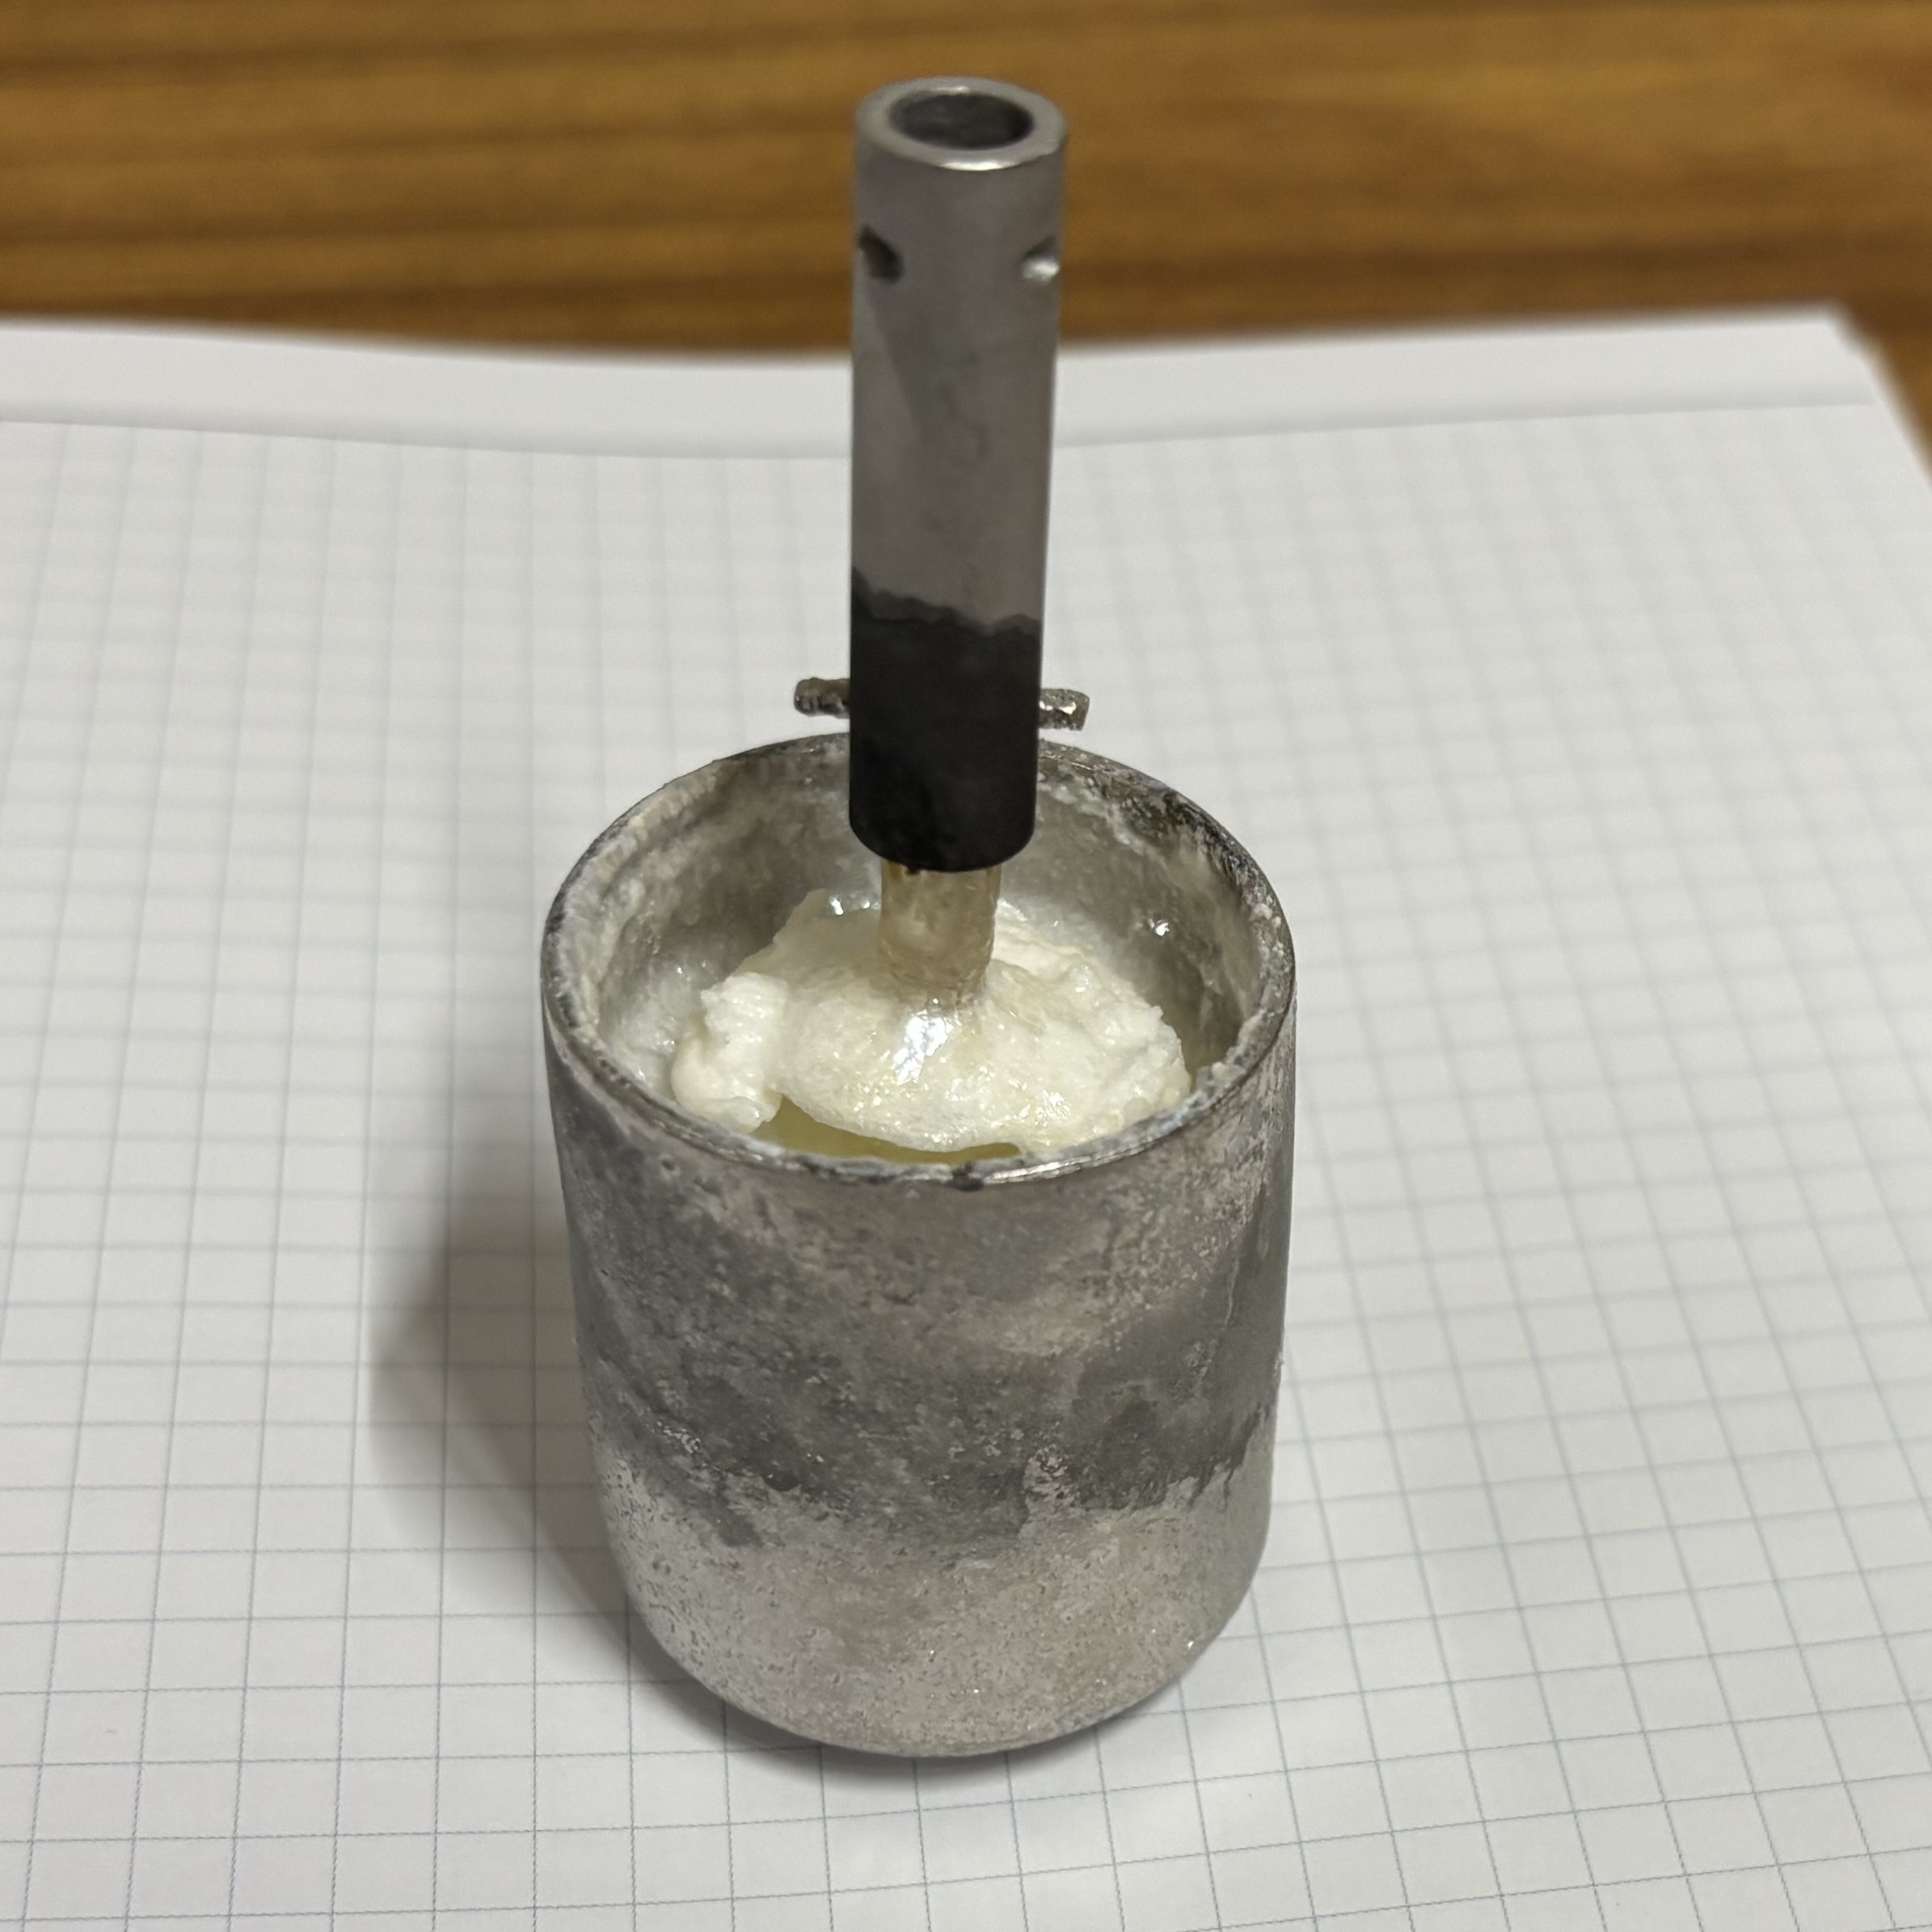
\includegraphics[width=\textwidth]{figures/Creuset avec agitateur.jpeg}
    \caption{View of the crucible with the embedded stirrer}
    \label{fig:img1}
\end{subfigure}
\hfill
\begin{subfigure}[b]{0.3\textwidth}
    \centering
    \includegraphics[width=\textwidth]{figures/Creuset YGG Vue de dessus.jpeg}
    \caption{Top view of the crucible}
    \label{fig:img2}
\end{subfigure}
\hfill
\begin{subfigure}[b]{0.3\textwidth}
    \centering
    \includegraphics[width=\textwidth]{figures/vue agitateur.jpeg}
    \caption{View of the stirrer after extraction}
    \label{fig:img3}
\end{subfigure}

\caption{Photographs of the crucible and the seed attached to the stirrer}
\label{fig:photos_assemb}
\end{figure}

Using a KEYENCE digital microscope, small transparent crystals were observed on the crucible walls. The surface of the solidified melt inside the crucible is heterogeneous (transparent, glassy, matte white), as shown in Figure \ref{fig:micro_assemb}.

\begin{figure}[H]
    \centering
    \includegraphics[width=0.4\linewidth]{figures/Creuset Flux Assemblage x20.jpg}
    \caption{Digital microscope image of the crucible containing the flux (magnification x20)}
    \label{fig:micro_assemb}
\end{figure}

\subsubsection{XRD results}
After analysing the powders collected at the crucible walls and near the seed, comparison of the two diffraction patterns shows that the same crystalline phase has grown on both surfaces (see Appendix). However, no YGG garnet could be detected.

\subsection{Results of growth tests in different fluxes}
After removal from the furnace, digital microscope observations were carried out to obtain more detailed images.

\begin{figure}[h]
\centering

\begin{subfigure}[b]{0.3\textwidth}
    \centering
    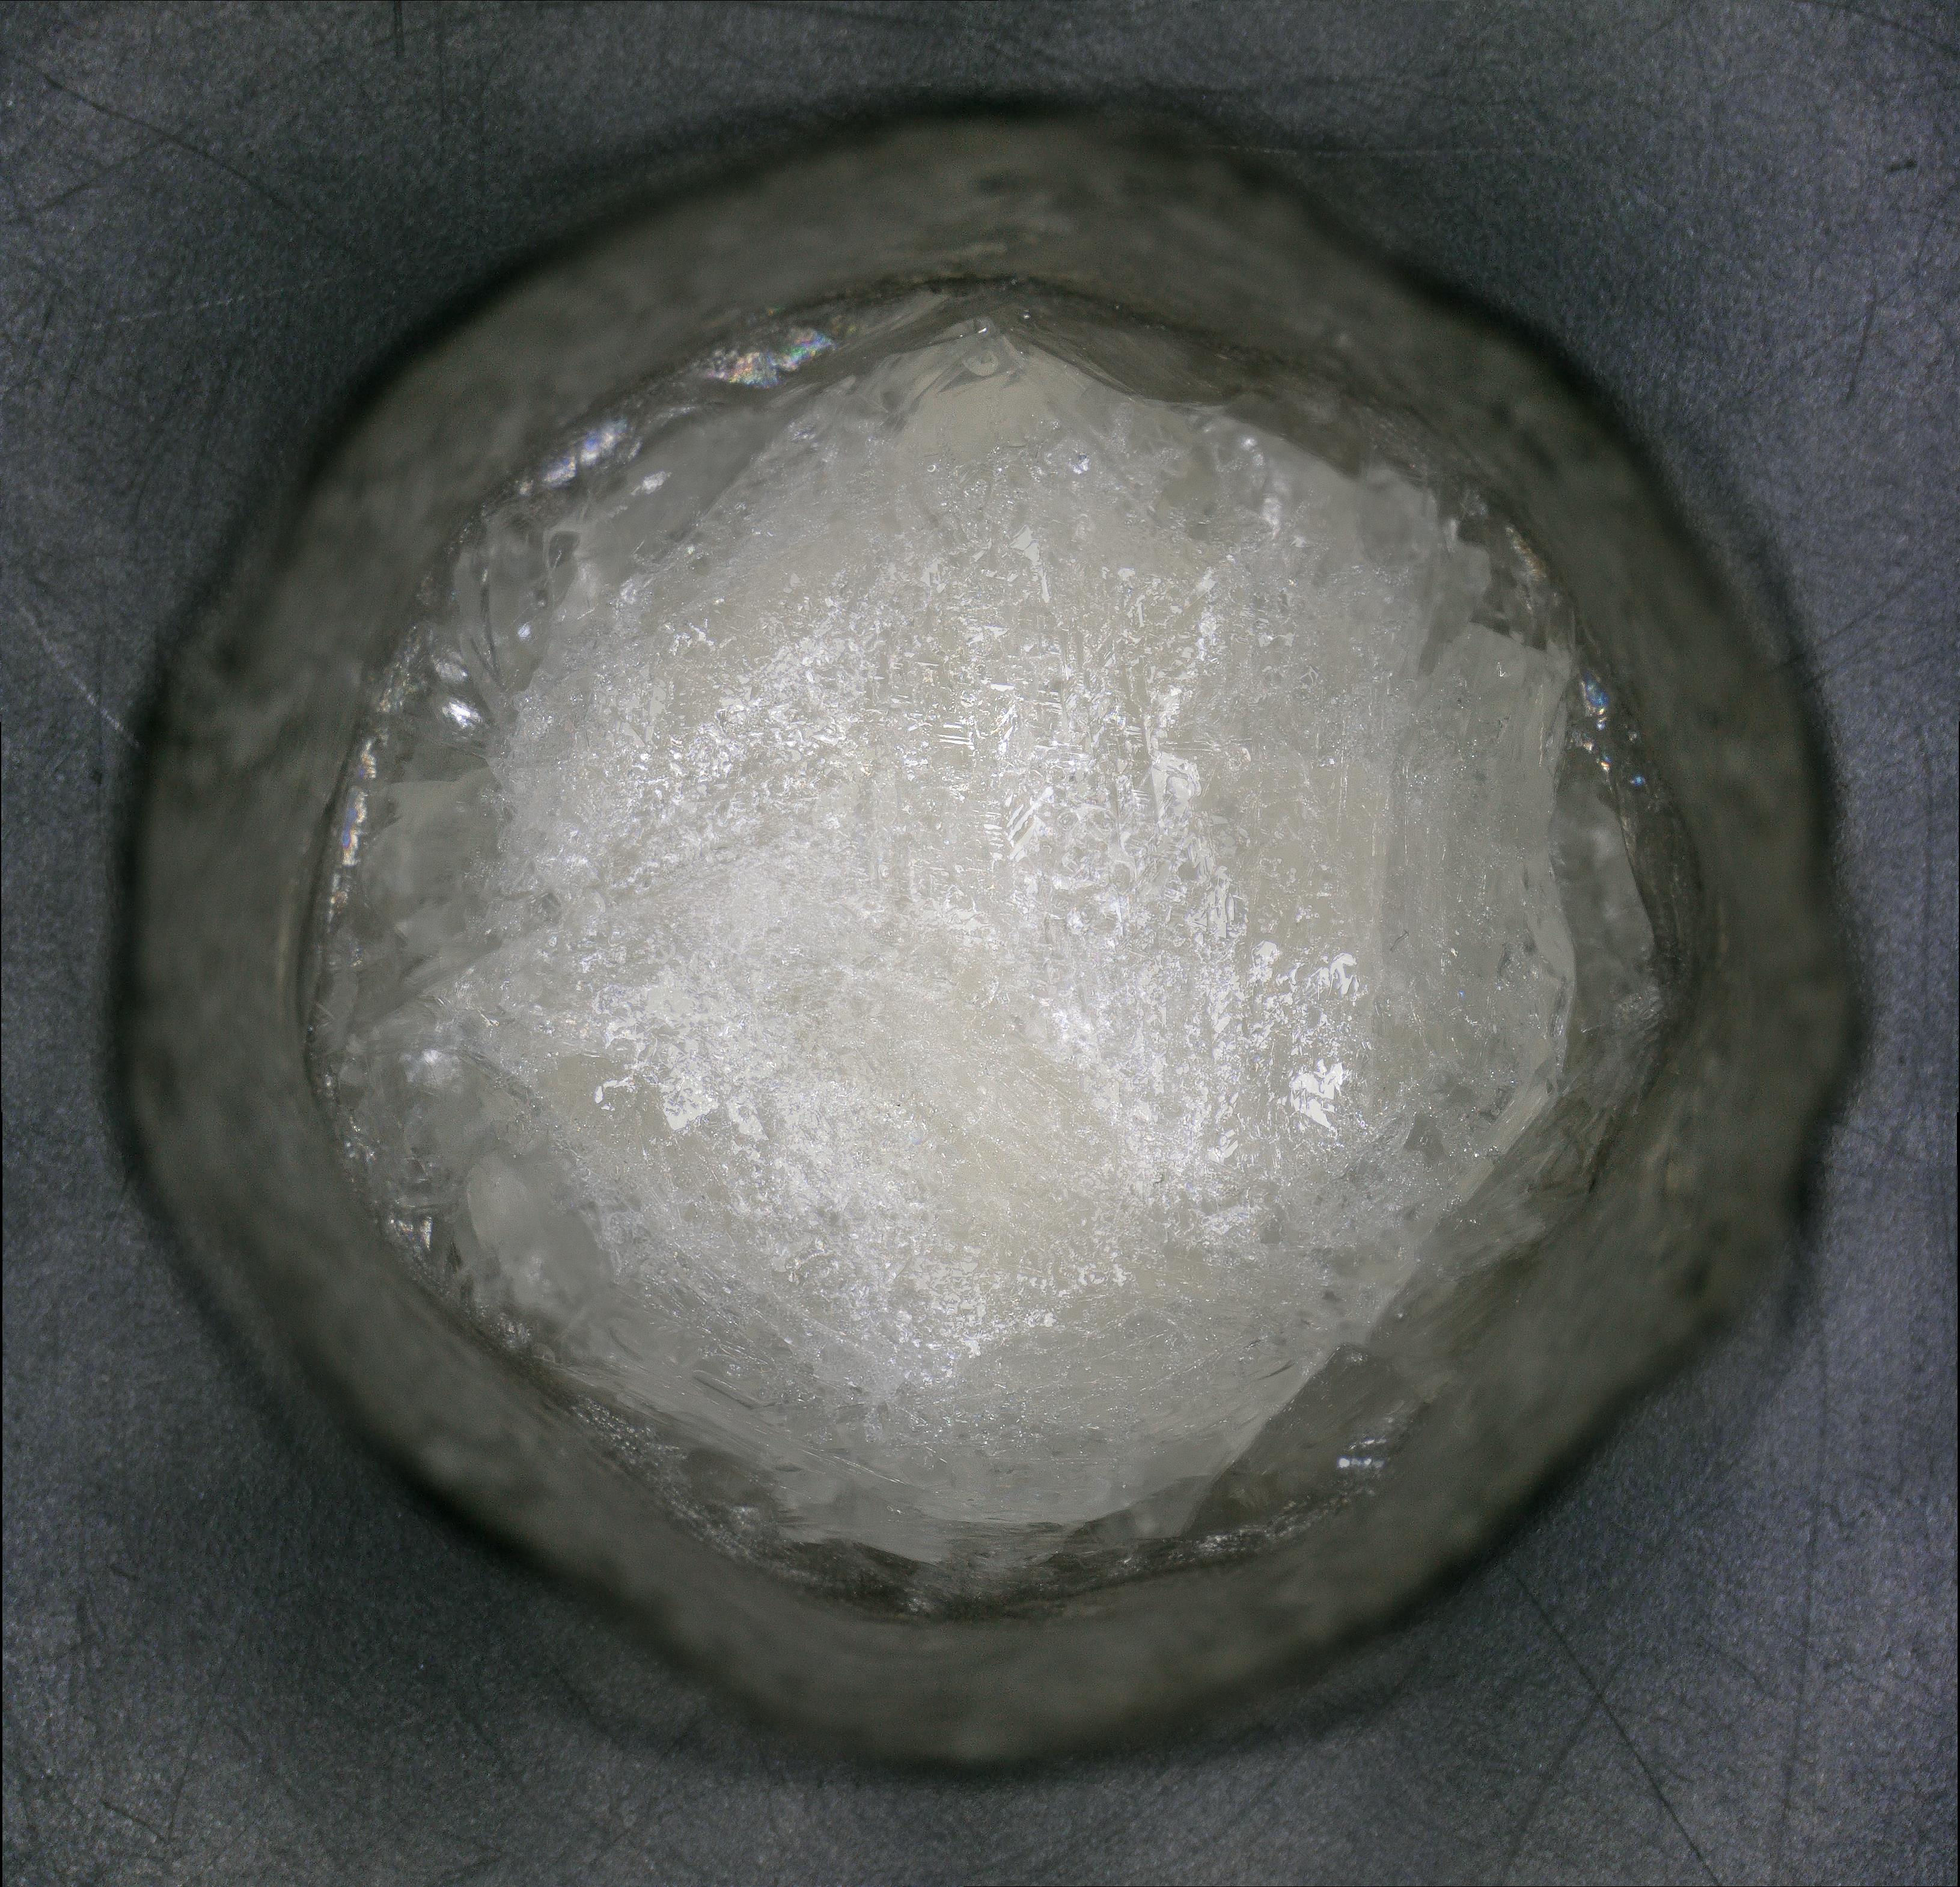
\includegraphics[width=\textwidth]{figures/Assemblage YGG x20.jpg}
    \caption{View of crucible [YGG]}
    \label{fig:img1}
\end{subfigure}
\hfill
\begin{subfigure}[b]{0.3\textwidth}
    \centering
    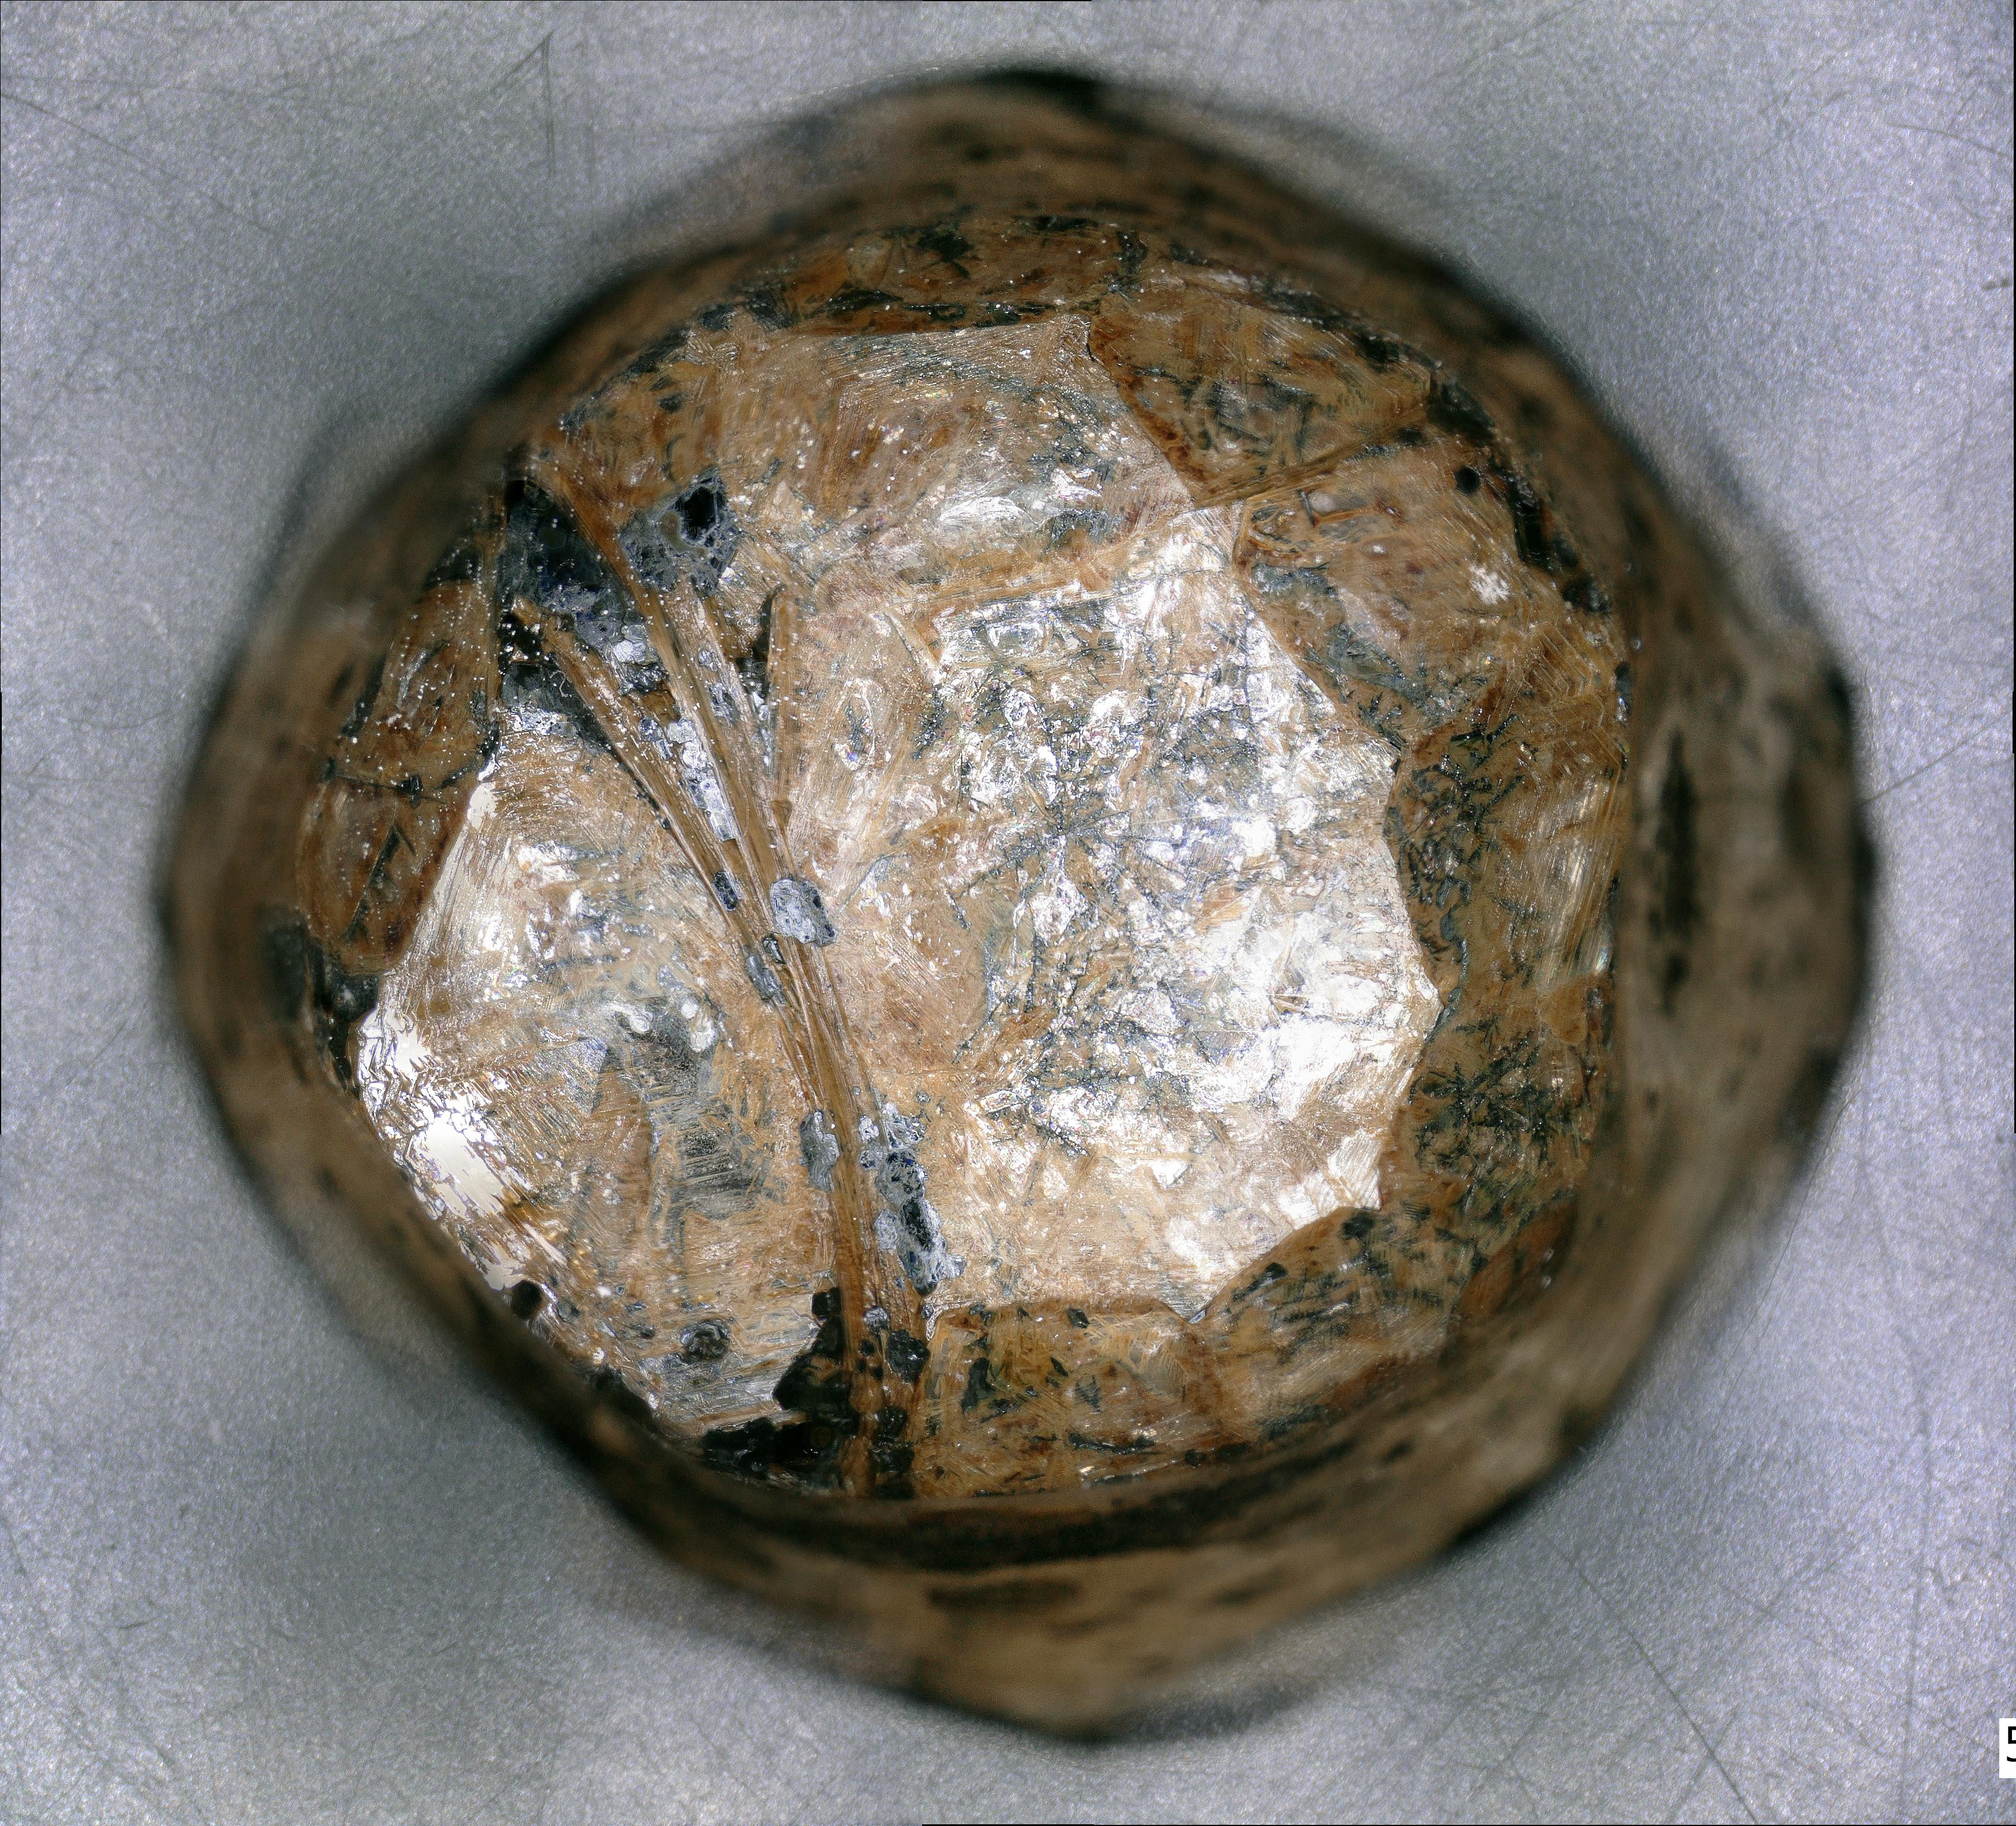
\includegraphics[width=\textwidth]{figures/Assemblage YIGG x20.jpg}
    \caption{View of crucible [YIGG]}
    \label{fig:img2}
\end{subfigure}
\hfill
\begin{subfigure}[b]{0.3\textwidth}
    \centering
    \includegraphics[width=\textwidth]{figures/Assemblage YIG x20.jpg}
    \caption{View of crucible [YIG]}
    \label{fig:img3}
\end{subfigure}

\caption{Digital microscope images of the three crucibles after removal from the furnace (magnification x20)}
\label{fig:photos_assemb}
\end{figure}

The content of crucible [YIGG] appears translucent with an orange tint and contains a number of black hexagonal crystals at the surface (Figure \ref{fig:YIGG-x50}).

\begin{figure}
    \centering
    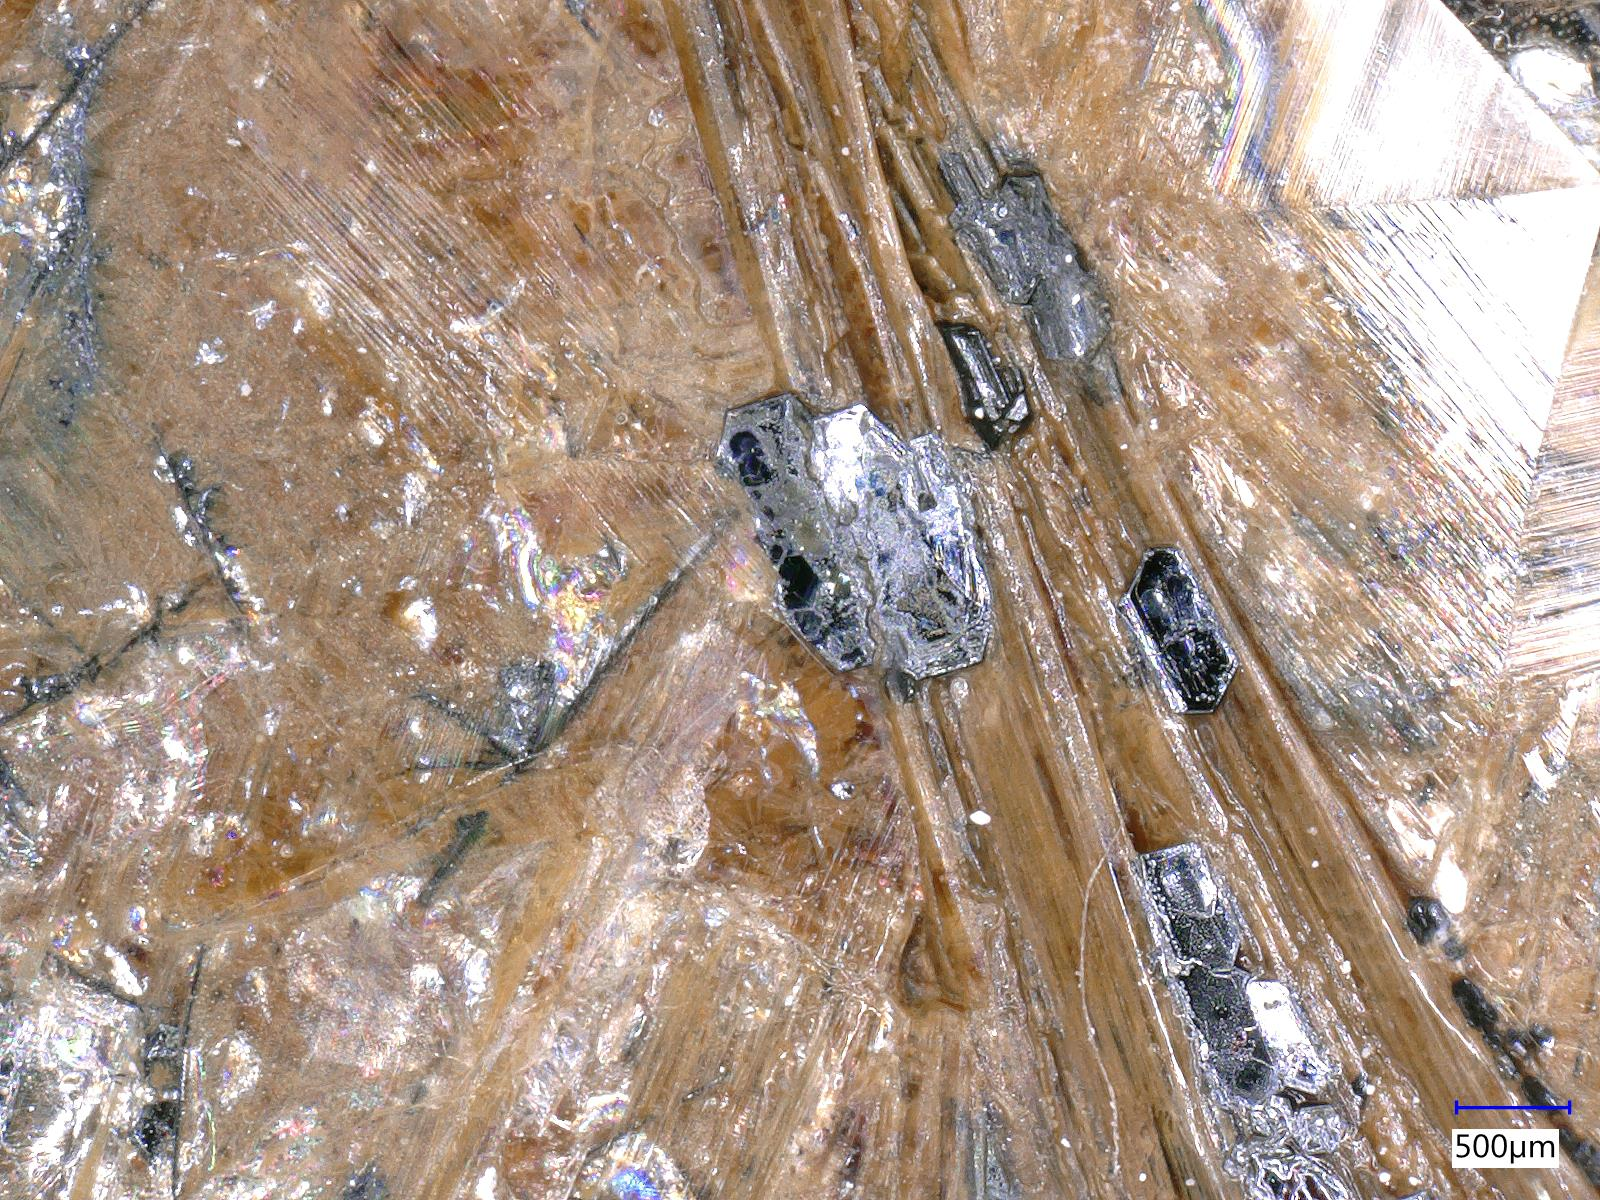
\includegraphics[width=0.5\linewidth]{figures/YIGG x50.jpg}
    \caption{Crystals visible to the naked eye on crucible [YIGG] (magnification x50)}
    \label{fig:YIGG-x50}
\end{figure}

The content of crucible [YIG] is an opaque black phase with striations at the surface (Figure \ref{fig:YIG_stries}). When illuminated, faint reddish spots can be seen. Small black hexagonal crystals are present at the surface (Figure \ref{fig:YIG_crist}). Although black crystals were observed, nothing yet confirms that they are garnets. This hypothesis is in fact unlikely given the crystal morphology observed in the two crucibles. Garnets crystallise in the cubic system, whereas the well-defined hexagonal platelets clearly indicate another nature. Considering the elements present in the crystallisation bath and the XRD results obtained on extracted samples, these crystals could belong to the $BaFeO_{3-x}$ family.

\begin{figure}[h]
    \centering

    \begin{subfigure}[t]{0.45\textwidth}
        \centering
        \includegraphics[width=\textwidth]{figures/YIG x50.jpg}
        \caption{View of surface striations (magnification x50)}
        \label{fig:YIG_stries}
    \end{subfigure}
    \hfill
    \begin{subfigure}[t]{0.45\textwidth}
        \centering
        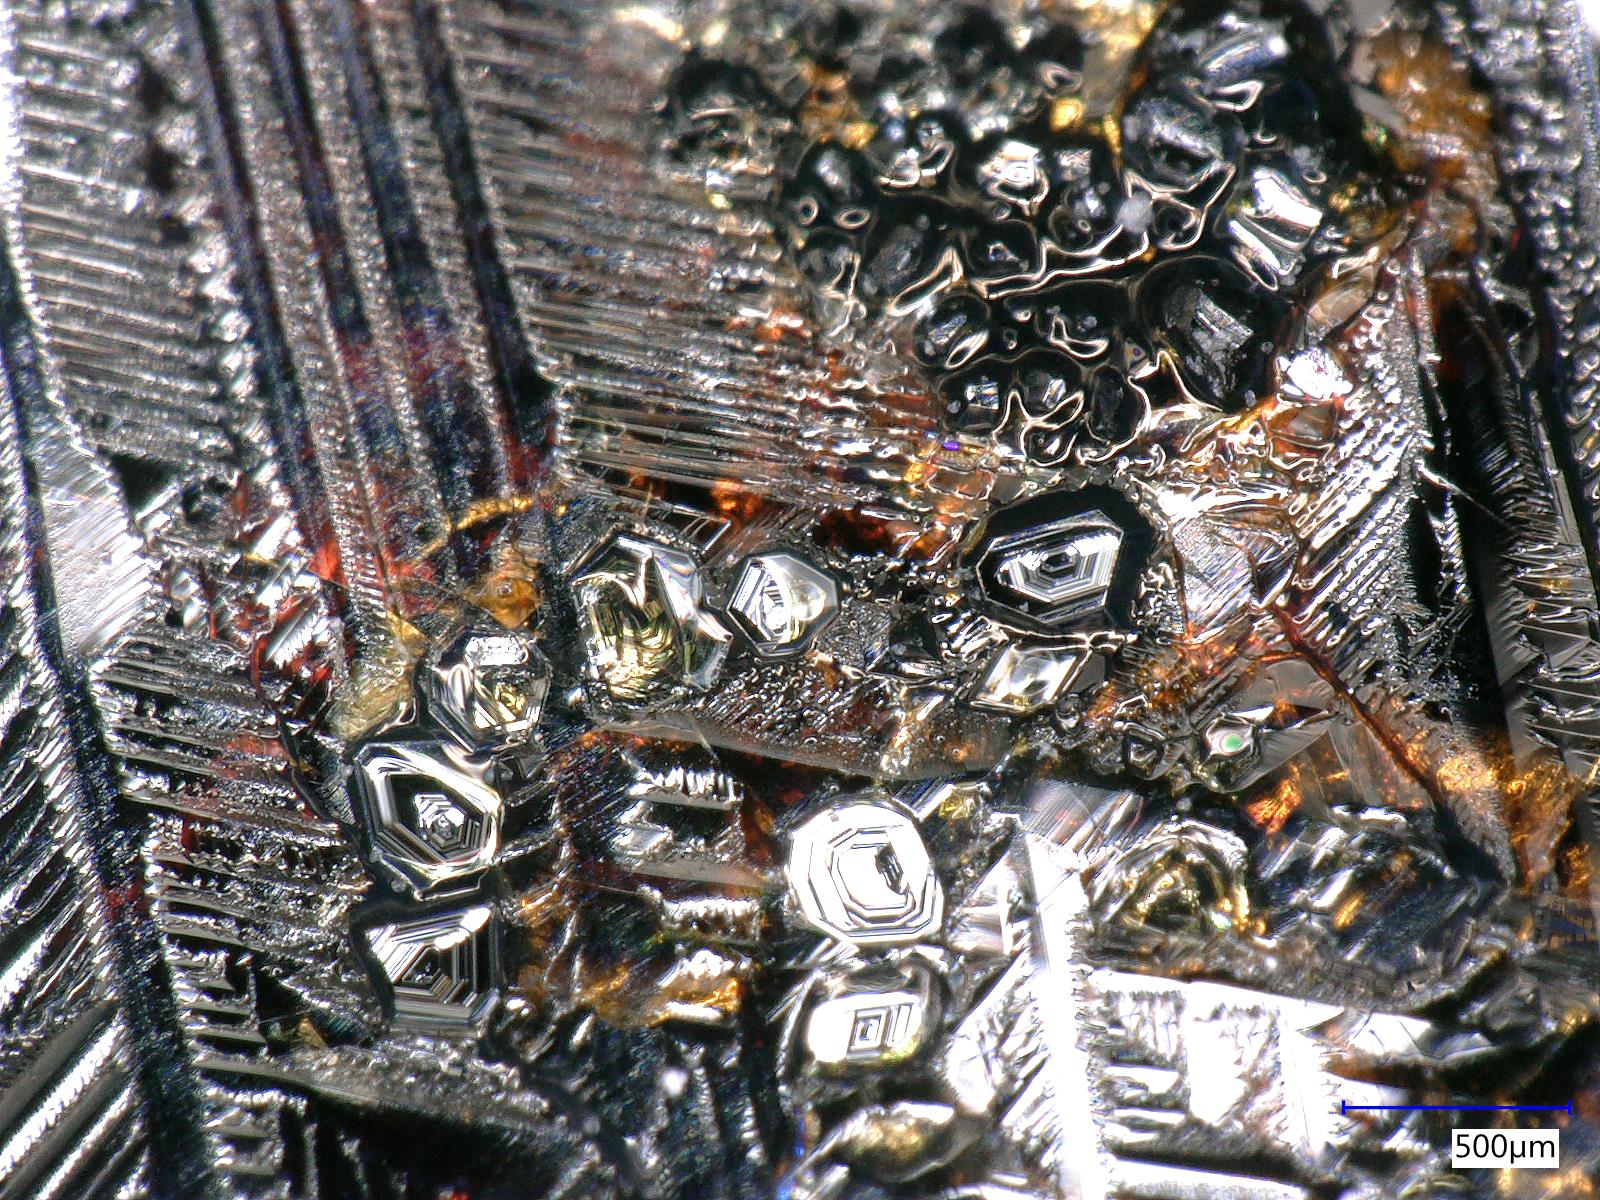
\includegraphics[width=\textwidth]{figures/YIG x100.jpg}
        \caption{View of hexagonal crystals (magnification x100)}
        \label{fig:YIG_crist}
    \end{subfigure}

    \caption{Details at the surface of crucible [YIG]}
    \label{fig:detail_YIG}
\end{figure}

Crucible [YGG] contains an inhomogeneous amorphous phase, translucent, transparent or matte white. Transparent or white crystals are observed at the surface and in deeper layers, together with opaque black solids (Figure \ref{fig:YGG-crist}).

\begin{figure}[H]
    \centering
    \includegraphics[width=0.5\linewidth]{figures/YGG x100.jpg}
    \caption{Crystals at the surface of crucible [YGG] and presence of black impurities}
    \label{fig:YGG-crist}
\end{figure}

The crystals present in the three crucibles could be recovered from the filter cake obtained after acid attack of the flux. In addition, crucible [YIG] shows, after acid treatment, a polycrystalline layer at the bottom, composed of crystals that may be cubic and therefore potentially correspond to the targeted garnet.

\begin{figure}[H]
    \centering
    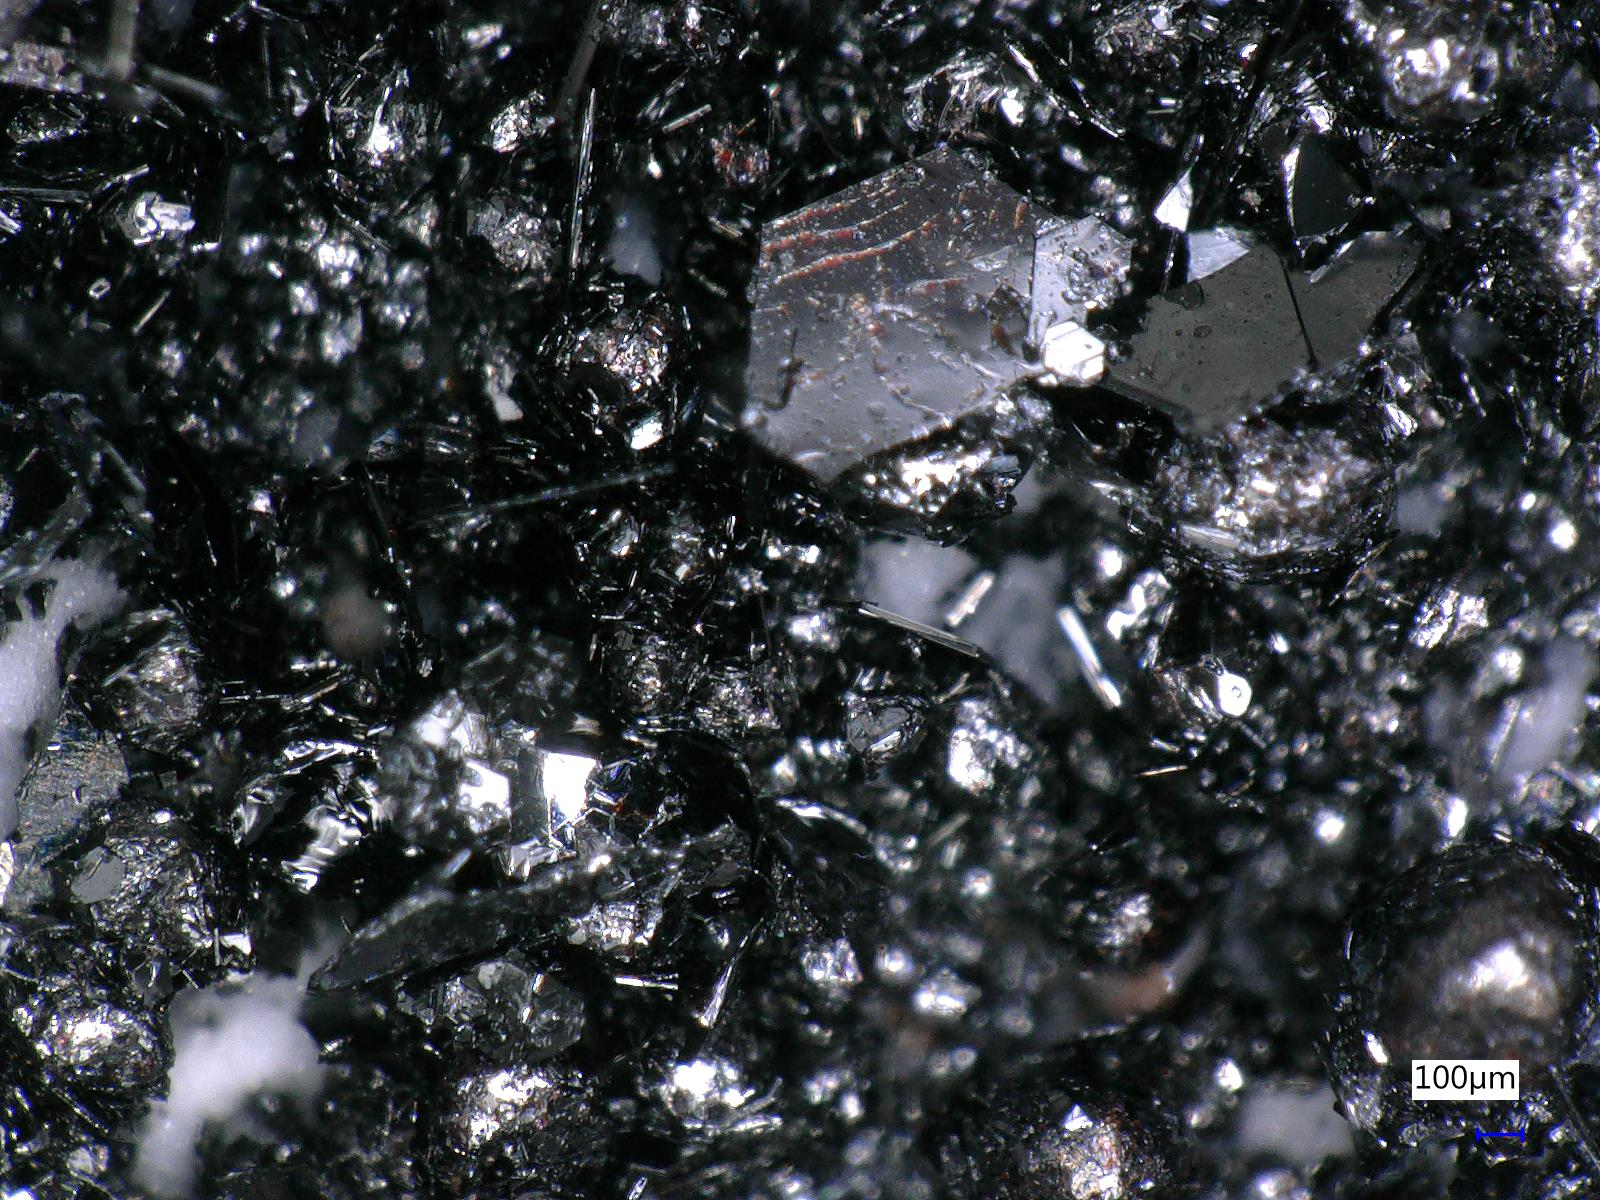
\includegraphics[width=0.5\linewidth]{figures/Creuset Post Acide YIGG x100.jpg}
    \caption{Crystals at the bottom of crucible [YIG] after acid attack}
    \label{fig:enter-label}
\end{figure}

The filter cake from crucible [YGG] shows transparent crystals together with a matte white amorphous phase and black matte solids. The filter cake from crucible [YIGG] contains a large amount of small (sub-millimetre) reflective black crystallites, as well as very small transparent white crystals that can be distinguished under the microscope. Finally, the filter cake from crucible [YIG] contains aggregates of larger black crystals, potentially cubic. These are surrounded by a green powder, corresponding to residual flux and iron that has reacted with nitric acid (ferric products in the $Fe^{2+}$ form). These details can be seen in the microscope images in Figure \ref{fig:micro_filtrats}.

\begin{figure}[H]
    \centering

    \begin{subfigure}[t]{0.3\textwidth}
        \centering
        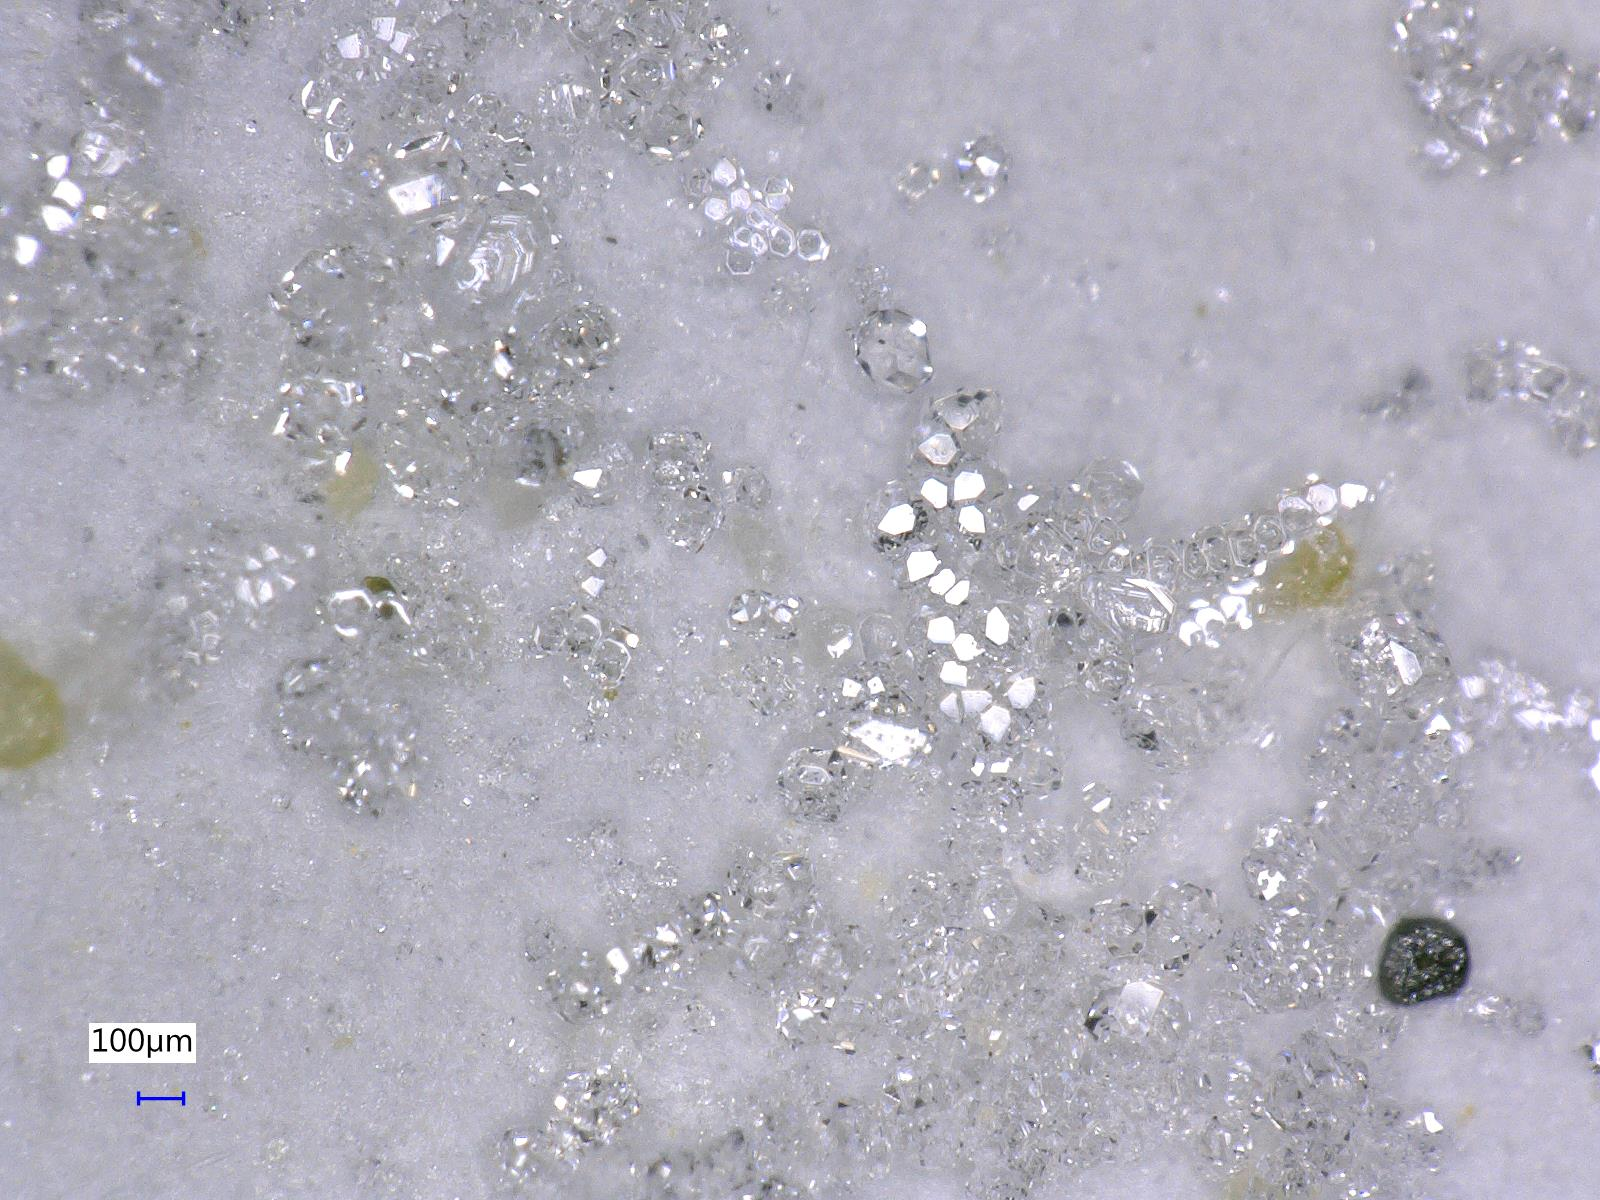
\includegraphics[width=\textwidth]{figures/Acide YGG x100.jpg}
        \caption{View of filter cake [YGG] (magnification x100)}
        \label{fig:YGG_filtrat}
    \end{subfigure}
    \hfill
    \begin{subfigure}[t]{0.3\textwidth}
        \centering
        \includegraphics[width=\textwidth]{figures/Acide YIGG x50.jpg}
        \caption{View of filter cake [YIGG] (magnification x100)}
        \label{fig:YIGG_filtrat}
    \end{subfigure}
    \hfill
    \begin{subfigure}[t]{0.3\textwidth}
        \centering
        \includegraphics[width=\textwidth]{figures/Acide YIG x200.jpg}
        \caption{View of filter cake [YIG] (magnification x100)}
        \label{fig:YIG_filtrat}
    \end{subfigure}

    \caption{Digital microscope images of the three filter cakes after acid attack}
    \label{fig:micro_filtrats}
\end{figure}

\subsubsection{XRD results}
For the three crucibles with 7.5 mol\% garnet, the XRD pattern of [YIG] is unambiguous: all observed peaks can be assigned to YIG. The diffractogram of crucible [YIGG] also confirms the presence of YIG, as suspected, but does not allow YGG to be identified. Parasite phases are also observed; these can be explained by the presence of nitrates in the filter cake originating from the nitric acid ($HNO_3$) used in the attack, which crystallised with the compounds present in the flux. The diffractogram of crucible [YGG] reveals similar parasite phases and does not confirm the presence of YGG.

However, flux growth of YGG garnet in this system is confirmed for a YGG fraction of 10 mol\%. The diffractogram of the fourth crucible indeed shows the presence of YGG in addition to a parasite phase, $Ba(NO_3)_2$.

\section{Conclusion}
This internship was carried out in the framework of ongoing research on flux growth of yttrium garnets, more specifically YIG and YGG. Two experimental approaches were implemented: an attempt at directed growth of a YGG single crystal by pulling from a seed, and a series of tests in different fluxes to study the influence of flux composition and garnet concentration on crystallisation. These experiments involved several preparation, chemical treatment and characterisation techniques (optical microscopy, acid attack, X-ray diffraction), which made it possible to observe and identify the phases obtained.

\subsection*{Main results}

Directed growth of a YGG single crystal from a $Gd_3Ga_5O_{12}$ seed did not lead to YGG formation, but instead produced a non-identified crystalline phase. This attempt highlights the current limitations of the pulling protocol used, which is probably not well suited to the crystallisation conditions of YGG. In parallel, experiments carried out in $BaO-B_2O_3-Na_2O$-based fluxes helped to better define the growth conditions for YIG, which appears relatively robust and is readily identified by XRD.

As for YGG, its crystallisation could be confirmed in the sodium-based flux for a garnet molar fraction increased to 10\%. At lower concentrations, no YGG could be detected. In the mixed [YIGG] system, although a wide variety of crystalline phases appears, the diffractograms do not clearly demonstrate the simultaneous presence of both garnets, due to peak overlap and possible competition between phases.

Overall, the results show that flux growth of YGG garnet is feasible but requires fine optimisation of both composition and experimental conditions. Increasing the garnet concentration seems to play a key role in promoting the selective precipitation of the desired phase. In addition, the nature of the parasite phases observed (notably nitrate-containing compounds resulting from the acid attack) underlines the importance of controlling every step of the protocol, including post-growth treatments.

Future work could focus on several aspects: fine-tuning the proportions of the flux components, improving control of the cooling profile, and exploring other seeds compatible with YGG to favour directed growth.

\section{Bibliography}
\begin{thebibliography}{17}

\bibitem{samuel} Internship report of Samuel Collange at IRCP-MPOE, 2024. 

\bibitem{mindat} Garnet Supergroup, Mindat, available at: \url{https://www.mindat.org/min-1651.html}.

\bibitem{azo} Nd:YAG Lasers Properties and Applications, AZO optics, 2013, available at: \url{https://www.azooptics.com/Article.aspx?ArticleID=470}.

\bibitem{chaneliere2014} Thierry Chanelière, A. Louchet-Chauvet, Alban Ferrier, Philippe Goldner, Cristaux et dispositifs optiques pour le traitement de l’information quantique, \textit{Techniques de l’ingénieur}, 2014.

\bibitem{musa2017} Makiyyu Abdullahi Musa, Raba’ah Syahidah Azis, Nurul Huda Osman, Jumiah Hassan, Tasiu Zangina, Structural and magnetic properties of yttrium iron garnet (YIG) and yttrium aluminum iron garnet (YAlG) nanoferrite via sol-gel synthesis, \textit{Elsevier}, 2017, available at: \url{http://dx.doi.org/10.1016/j.rinp.2017.02.038}.

\bibitem{usami2011} N. Usami, Types of silicon–germanium (SiGe) bulk crystal growth methods and their applications, \textit{Elsevier}, 2011, available at: \url{https://doi.org/10.1533/9780857091420.2.72}.

\bibitem{lohfeld2005} Stefan Lohfeld, M. Schütze, Oxidation behaviour of particle reinforced MoSi$_2$ composites at temperatures up to 1700°C. Part II: Initial screening of the oxidation behaviour of MoSi$_2$ composites, \textit{Materials and Corrosion}, 2005, available at: \url{http://dx.doi.org/10.1002/maco.200403832}.

\bibitem{morris1979} A.W. Morris, D. Elwell, High temperature solution growth of yttrium aluminium garnet crystals using accelerated crucible rotation, \textit{Journal of Material Science}, 1979, available at: \url{https://doi.org/10.1007/BF00688418}.

\bibitem{hiskes1974} R. Hiskes, LPE growth and characterization of magnetic garnets grown in BaO-based solvents, \textit{Journal of Crystal Growth}, 1974, available at: \url{https://doi.org/10.1016/S0022-0248(74)80076-X}.

\bibitem{levin1949} Ernest M. Levin, Howard F. McMurdie, The system BaO-B$_2$O$_3$, \textit{Journal of the American Ceramic Society}, 1949, available at: \url{http://dx.doi.org/10.1111/j.1151-2916.1949.tb18932.x}.

\bibitem{laudise1962} R.A. Laudise, R.C. Linares, E.F. Dearborn, Growth of Yttrium Iron Garnet on a Seed from a Molten Salt Solution, \textit{Journal of Applied Physics}, 1962, available at: \url{https://doi.org/10.1007/978-1-4899-6391-8_144}.

\bibitem{elwell1974} D. Elwell, P. Capper, C.M. Lawrence, Viscosity and density of BaO/B$_2$O$_3$/BaF$_2$ fluxes and solutions, \textit{Journal of Crystal Growth}, 1974.

\bibitem{feigelson1990} R.S. Feigelson, R.J. Raymakers, R.K. Route, Growth of nonlinear crystals for frequency conversion, \textit{Progress in Crystal Growth and Characterization of Materials}, 1990, available at: \url{https://doi.org/10.1016/0960-8974(90)90022-K}.

\bibitem{fedorov2002} P.P. Fedorov, A.E. Kokh, N.G. Kononova, Barium borate $\beta$-BaB$_2$O$_4$ as a material for nonlinear optics, \textit{Russian Chemical Reviews}, 2002, available at: \url{http://dx.doi.org/10.1070/RC2002v071n08ABEH000716}.

\bibitem{timofeeva1981} V.A. Timofeeva, A.B. Bykov, V.S. Nikolov, Phase equilibria in BaO-B$_2$O$_3$-BaF$_2$-Y$_2$O$_3$-Fe$_2$O$_3$ system, \textit{Journal of Crystal Growth}, 1981, available at: \url{https://doi.org/10.1016/0022-0248(81)90354-7}.

\bibitem{suemune1974} Y. Suemune, N. Inoue, Crystallization of garnets in BaO-BaF$_2$-B$_2$O$_3$ solvents, \textit{Journal of Crystal Growth}, 1974, available at: \url{https://doi.org/10.1016/0022-0248(74)90397-2}.

\bibitem{capper1974} P. Capper, D. Elwell, Appraisal of BaO/B$_2$O$_3$/BaF$_2$ fluxes for the growth of yttrium aluminium garnet, \textit{Journal of Crystal Growth}, 1974, available at: \url{https://doi.org/10.1016/0022-0248(74)90202-4}.

\end{thebibliography}
\newpage
\section{Appendices}
\setcounter{figure}{0}
\appendix
\section{Furnace programmes}
\label{annexe:programme_four}
\begin{figure}[p]
    \centering
    \includegraphics[width=\textwidth,keepaspectratio]{figures/Programme_temp_flux.png}
    \caption{Furnace programme for the $0.4BaO - 0.3B_2O_3 - 0.3BaF_2$ flux}
    \label{fig:programme_temp_flux}
\end{figure}
\begin{figure}[p]
    \centering
    \includegraphics[width=\textwidth,keepaspectratio]{figures/Programme_temp_flux.png}
    \caption{Furnace programme for the $0.4BaO - 0.3B_2O_3 - 0.3BaF_2$ flux}
    \label{fig:programme_temp_flux}
\end{figure}
\newpage
\section{XRD results}
\begin{figure}[htbp]
    \centering
    \includegraphics[width=\textwidth]{figures/Ka1_spin_flux433_4pcYGG_centre et bord.pdf}
    \caption{Comparison between the diffractograms of the samples collected on the seed (blue) and at the crucible walls (red)}
    \label{fig:exemple-pdf}
\end{figure}

\begin{figure}[htbp]
    \centering
    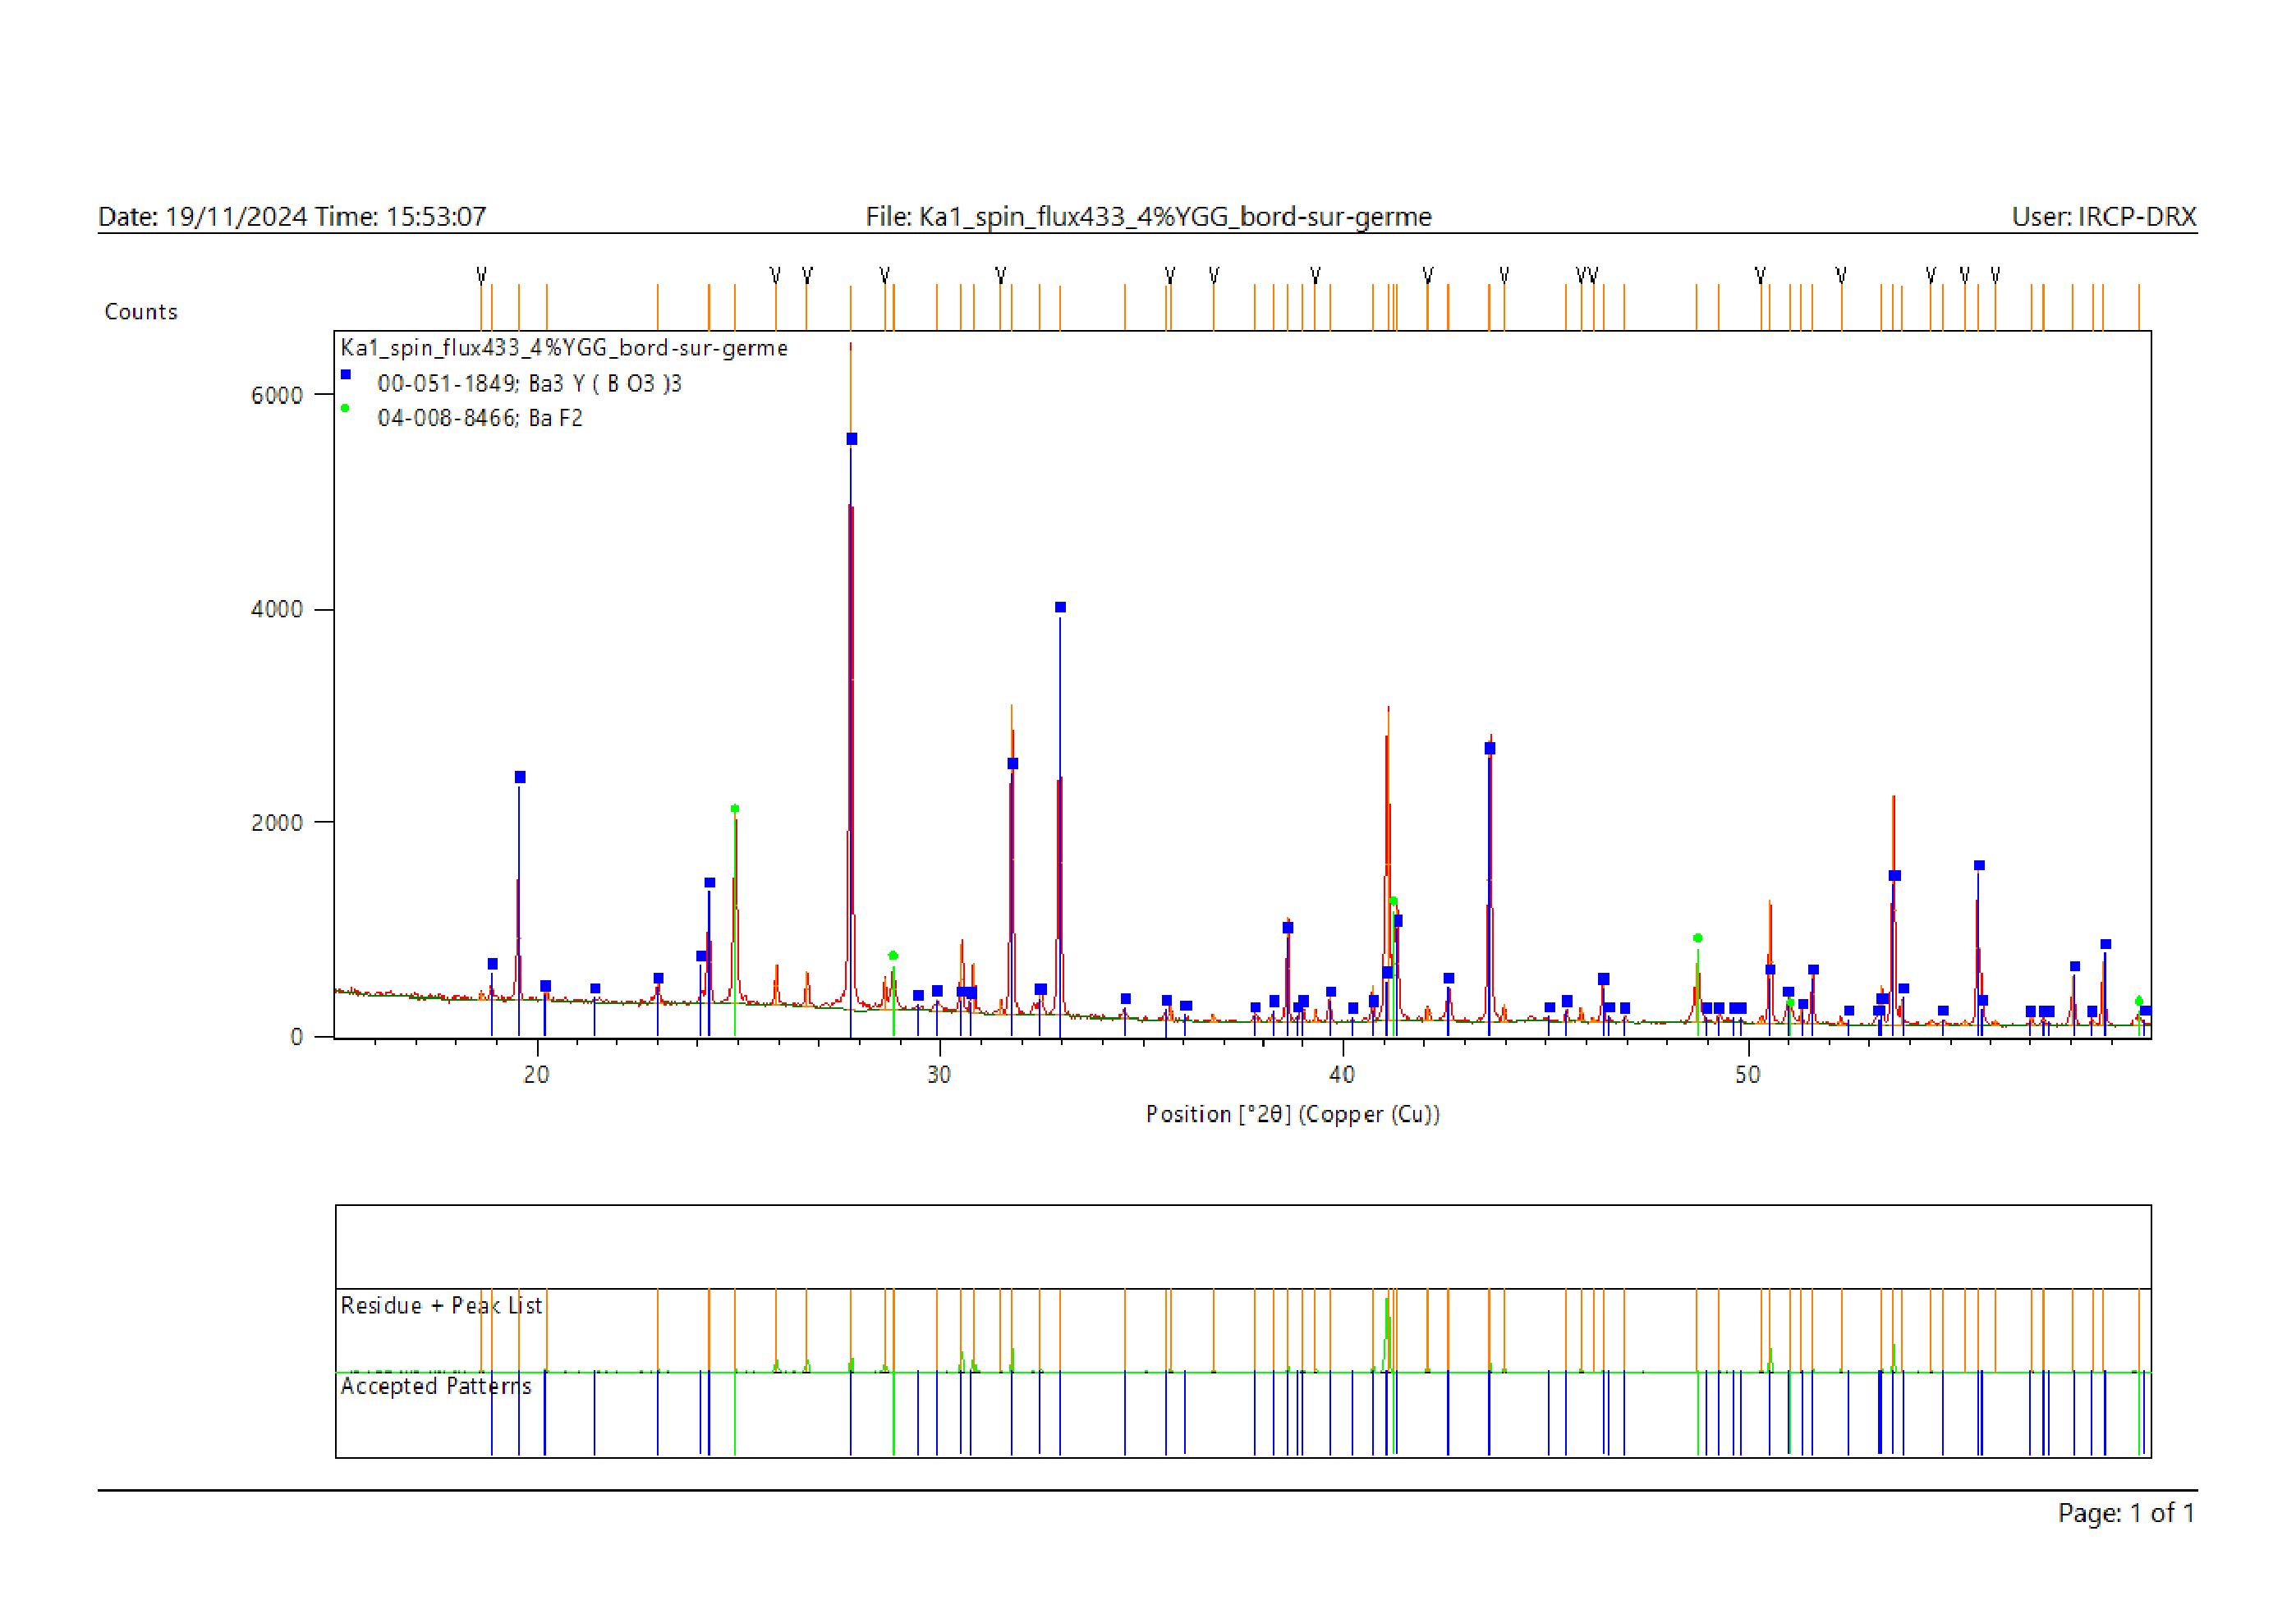
\includegraphics[width=\textwidth]{figures/Ka1_spin_flux433_4pcYGG_bord-sur-germe.pdf}
    \caption{Diffractogram of the crystals at the walls of the pulling crucible}
    \label{fig:exemple-pdf}
\end{figure}

\begin{figure}[htbp]
    \centering
    \includegraphics[width=\textwidth]{figures/Ka1_spin_flux433_4pcYGG_centre-sur-germe.pdf}
    \caption{Diffractogram of the crystals on the seed in the pulling crucible}
    \label{fig:exemple-pdf}
\end{figure}

\begin{figure}[htbp]
    \centering
    \includegraphics[width=\textwidth]{figures/Ka1_spin_flux433_4pccreusetYIGG.pdf}
    \caption{Diffractogram of the crystals formed in crucible [YIGG]}
    \label{fig:exemple-pdf}
\end{figure}

\begin{figure}[htbp]
    \centering
    \includegraphics[width=\textwidth]{figures/Ka1_spin_flux433_4pccreusetYIG.pdf}
    \caption{Diffractogram of the crystals formed in crucible [YIG]}
    \label{fig:exemple-pdf}
\end{figure}

\end{document}
